
\begin{landscape}

    \begin{figure}[h]
    \centering
    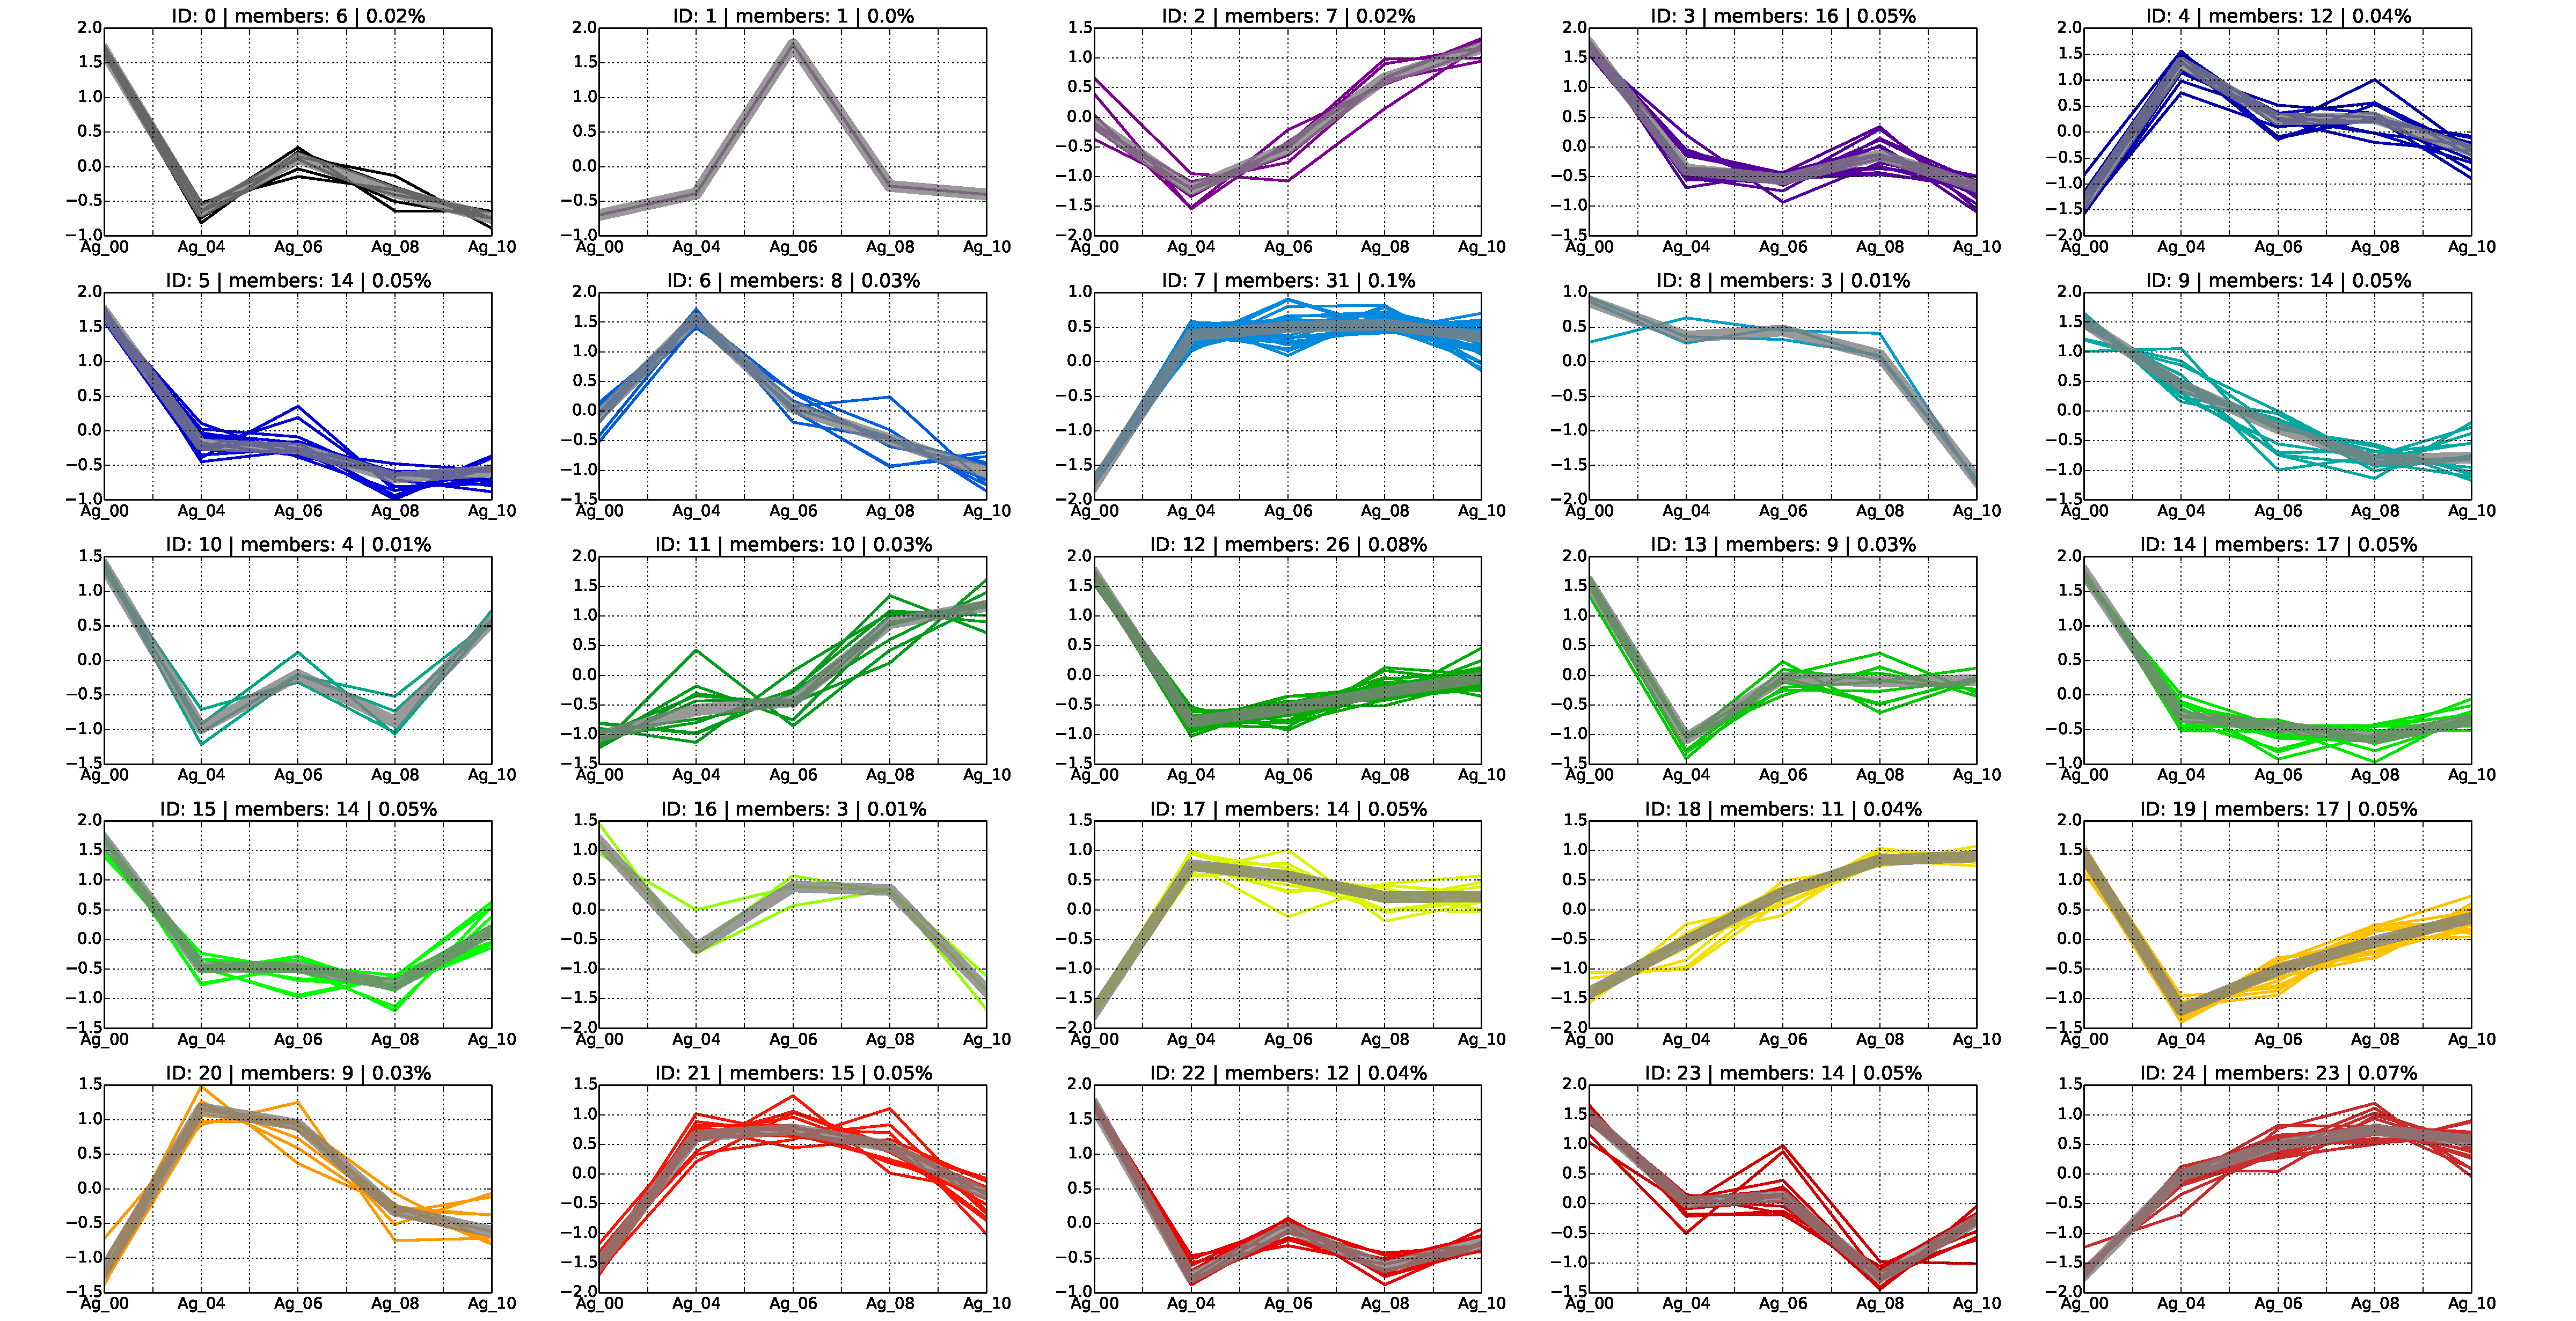
\includegraphics[width=\linewidth]{figures/figs/ecr_and_insects_ptci_20130903/ecr_and_insects_ptci1_gene_profiles_from_cummerbund/25_clusters.pdf}
    \caption[\Ag\ clustered abundance profiles]{\sf \textbf{\Ag\ clustered abundance profiles.} \\ 
    Clusters were generated using k-means clustering as implemented in Biopython version 1.62 \cite{Cock2009}.  Abundance profile data was log transformed after one FPKM was added to all data to remove zeros ($log_{10}(\mathrm{FPKM}+1)$).  K-means was then applied using the arithmetic mean as the center for cluster definition.  The data displayed here is the gene-wise standardization of the \textbf{raw} FPKM data such that each profile has mean = 0 and standard deviation = 1. Each median abundance profile is marked by a thick gray line. \textbf{Panel Titles} - ID: cluster identifier | members: number of genes in cluster | percentage of genes represented in all clusters. \textbf{Time Points} - \gls{NBF}, 4, 6, 8, 10 h \gls{PBM}.
}
    \label{fig:25-clusters}
    \end{figure}
    
\end{landscape}

